\section{Software Architecture}
This chapter describes the solution developed during our work. At the beginning the software architecture will be explained, followed by the partial steps and experiments which were needed to find the solution.
\\\\
The software architecture has to fulfil multiple requirements for this project. It should be easily extendable with new algorithms and ui extensions. The input and output format of the application should be independent from the algorithms and the ui to use different file types like bitmap images or \Gls{DXF}/\Gls{DWG} formats. The algorithms of the application should be link together as workflows which then can be executed by an engine in parallel.

\begin{figure}
  \centering
      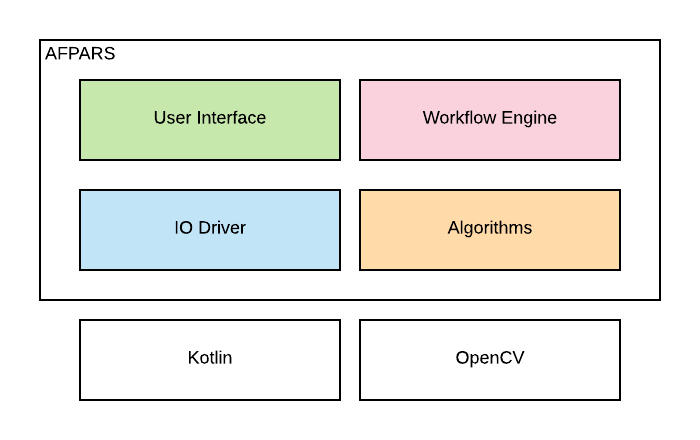
\includegraphics[width=0.8\textwidth]{AFPARS_Architecture}
  \caption{AFPARS software architecture.}
\end{figure}

\todo{Requirement - Solution}

\subsection{Meta Format}
To support the different input and output formats the architecture uses a meta format for the
floor plans called AFImage.
\subsection{Algorithm}
\subsection{Workflow}

\subsection{User Interface}
\missingfigure{User Interface Image.}
\todo{Why it looks like that. (Andere Software)}